\documentclass[border=1pt]{standalone}
% packages
\usepackage{tikz}
\usepackage{tikz-qtree}
\usetikzlibrary{positioning,quotes,calc,arrows.meta,shapes}
% tikz setup
\tikzset{%
  arrow/.style = {
    ->,
    > = latex,
    very thick,
    rounded corners,
    fill = #1,
    draw = #1,
  },
  wide/.style = {
    line width = #1,
  },
  tbox/.style = {
    thick,
    rounded corners,
    fill = #1!20!white,
    draw = #1!80!white,
    align = center,
    minimum width = 0.8cm,
    minimum height = 0.6cm,
    node distance = 1.5cm,
  },
  branch/.style = {
    grow = down,
    thick,
    rounded corners = 0.1cm,
    fill = #1!20!white,
    draw = #1!80!white,
    align = center,
    minimum width = 3cm,
    minimum height = 1cm,
    node distance = 1cm,
  },
  branch/.default = {gray},
  leaf/.style = {
    grow = down,
    thick,
    rounded corners = 0.35cm,
    fill = #1!20!white,
    draw = #1!80!white,
    align = center,
    minimum width = 0.7cm,
    minimum height = 0.7cm,
    font = \normalfont,
  },
  leaf/.default = {blue},
}
% selectors
\definecolor{all}     {RGB}{  0,  0,  0}
\definecolor{S}       {RGB}{  0,153,255}
\definecolor{I}       {RGB}{204, 51,  0}
\definecolor{T}       {RGB}{204, 51,153}
\definecolor{infected}{RGB}{204,  0, 51}
\definecolor{High}    {RGB}{ 34, 34, 34}
\definecolor{Med}     {RGB}{ 85, 85, 85}
\definecolor{Low}     {RGB}{187,187,187}
% from beamer
\definecolor{C1}{HTML}{224466}
\definecolor{C2}{HTML}{CC3300}
\definecolor{C3}{HTML}{666666}

% colors
\newcommand{\colorx}{C1}
\newcommand{\colort}{\colorx!50!black}
\newcommand{\colorw}{\colorx}
% document
\begin{document}
\begin{tikzpicture}[
  pie/.style = {
    anchor=center,
    node distance=0.8cm,
  },
  wisp/.style = {
    draw = \colorw,
    fill = \colorw,
    thick,
  },
]
% nodes ----------------------------------------------------------------------------------------
\node(x1) [tbox=\colorx] at (0.0,0.0)          {$H$};
\node(x3) [tbox=\colorx, below = 0.5cm of x1]  {$L$};
\coordinate (x2) at ($(x1)!0.5!(x3)$);
\coordinate[left  = 1cm of x2](x2a) ;
\coordinate[right = 1cm of x2](x2b);
% arrows ---------------------------------------------------------------------------------------
\draw[arrow=\colort,wide=\turnover,fill=none,-{Latex[length=4mm]}] (x3) -| (x2a) |- (x1); 
\draw[arrow=\colort,wide=\turnover,fill=none,-{Latex[length=4mm]}] (x1) -| (x2b) |- (x3);
% pies -----------------------------------------------------------------------------------------
\node(p13) [pie, right of = x2b] {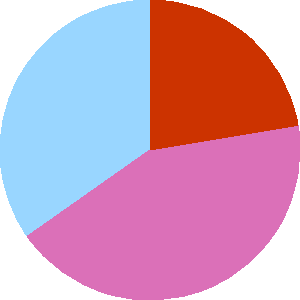
\includegraphics[width=1.25cm]{flow-high}};
\node(p31) [pie, left  of = x2a] {\includegraphics[width=1.25cm]{flow-low}};
\node(c13)[draw=\colorw,thick,circle,minimum width=1cm] at (p13) {};
\draw[wisp] (x2b) -- (c13.165) -- (c13.195)  -- cycle;
\node(c31)[draw=\colorw,thick,circle,minimum width=1cm] at (p31) {};
\draw[wisp] (x2a) -- (c31.15) -- (c31.345)  -- cycle;
\end{tikzpicture}
\end{document}
% eof
